\documentclass[aspectratio=169]{beamer}
\mode<presentation>{\usetheme{Warsaw}}
\mode<presentation>{\usefonttheme{professionalfonts}}

\usepackage{tikz,tkz-euclide}
%\usetikzlibrary{decorations.pathreplacing}
\usepackage{adjustbox}
\usepackage{mathtools, siunitx}
\usepackage{xcolor}

%\usefonttheme[onlymath]{serif}
\title{Beam Laydown in Satellite System Loading}
\institute{Copiam}
\author{Cham Kchao}
\date{May 6, 2020}

\setbeamertemplate{footline}{%
  \leavevmode%
%  \hbox{\begin{beamercolorbox}[wd=.5\paperwidth,ht=2.5ex,dp=1.125ex,leftskip=.3cm plus1fill,rightskip=.3cm]{author in head/foot}%
%    \usebeamerfont{author in head/foot}\insertshortauthor~(\insertshortinstitute)
  \hbox{\begin{beamercolorbox}[wd=.5\paperwidth,ht=2.5ex,dp=1.125ex,leftskip=.3cm,rightskip=.3cm plus1fil]{author in head/foot}%
    \usebeamerfont{author in head/foot}\insertshortdate\hfill\insertshortauthor~(\insertshortinstitute)
  \end{beamercolorbox}%
  \begin{beamercolorbox}[wd=.5\paperwidth,ht=2.5ex,dp=1.125ex,leftskip=.3cm,rightskip=.3cm plus1fil]{title in head/foot}%
%    \usebeamerfont{title in head/foot}\insertshorttitle\hfill\insertframenumber\,/\,\inserttotalframenumber
    \usebeamerfont{title in head/foot}\insertshorttitle\hfill\insertframenumber\
  \end{beamercolorbox}}%
  \vskip0pt%
}

%\setbeamertemplate{itemize item}[square]
\setbeamertemplate{itemize subitem}[square]
\setbeamerfont{itemize/enumerate subbody}{size=\small}



\begin{document}
\addtocounter{framenumber}{1}
\maketitle

\section{Introduction}
\begin{frame}
\frametitle{Background and Motivation}
Back in 2007, I was working on the TSAT program/SE\&T team
\begin{itemize}
\item Space segments had loading tools.  The Aerospace team had their tool.
\item We did not have a viable loading tool ... and a loading tool needs to laydown beams.
\end{itemize}
There are a variety of scenarios that necessitate the determination of antenna pointing locations
\begin{itemize}
\item To maximize the number of terminals within an antenna coverage

\item To maximize the throughpout within an antenna coverage or of a constellation
\item To meet a specified coverage of particular users (e.g. disadvantage users)
\end{itemize}
We will look at an approach that provides a set of {\em optimal} pointing locations
\begin{itemize}
\item based on maximizing the number of termianls within an antenna coverage
\item could be extended to other criteria.
\end{itemize}
\end{frame}

\section{Pointing Coordinate}
\subsection{Rational}
\begin{frame}
\frametitle{Pointing Coordinate - Simplified Approach with Circular Beam Pattern}
\begin{columns}

\column{0.6\textwidth}
\begin{itemize}
\item With a circular beam, a pair of terminals would lead to two possible pointing coordinates.
\begin{itemize}
	\item One defined by the green circle and one defined by the reflection about the line joining the locations of the terminal pair.
	\item A similar approach can be applied to an elliptical beam.
\end{itemize}
\item A list of all terminal pairs, along with coordinates of circle centers, allows for the determination of optimal pointing.
\end{itemize}
\column{0.4\textwidth}
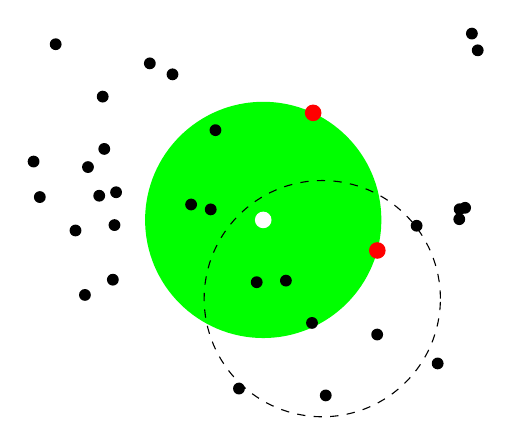
\begin{tikzpicture}[scale=0.5,every node/.style={scale=0.7}]
\def\rx{6}
\def\ry{5}
\def\r{3}
\fill[green] (0,0) circle [radius=\r cm];
\coordinate (O) at (0,0);
\path (O) +(-15:\r) coordinate (A);
\path (O) +(65:\r) coordinate (B);
\fill[red] (A) circle (6pt);
\fill[red] (B) circle (6pt);
\fill[white] (O) circle (6pt);

\draw[dashed] (1.5,-2) circle [radius=\r cm];

\foreach \x in {1,2,...,30}{
	\coordinate (A) at (rand*\rx, rand*\ry);
	\fill[black] (A) circle [radius=0.15 cm];
}


\end{tikzpicture}
\end{columns}

\end{frame}

\subsection{Options}
\begin{frame}
\frametitle{Pointing Coordinate - in 2D Cartesian System}
\begin{columns}

\column{0.5\textwidth}
One option is to solve the following two non-linear equations for $(c_x, c_y)$
\[ (c_x-x_1)^2 + (c_y-y_1)^2 = {r}^2 \]
and
\[  (c_x-x_2)^2 + (c_y-y_2)^2 = r^2 \,. \]
 It would result in long expressions with many operations for $c_x$ and $c_y$.
\column{0.5\textwidth}
\begin{tikzpicture}[scale=0.5,every node/.style={scale=1}]
\def\r{4}
\tkzDefPoints{0/0/A, 6/2/B}
%\tkzDrawCircle[R](A,\r cm)
\fill[green] (A) circle [radius=\r];
\tkzDrawCircle[R,dashed](B,\r cm)
\tkzInterCC[R](A, \r cm)(B, \r cm)  \tkzGetPoints{X}{Y}
\tkzInterLL(A,B)(X,Y) \tkzGetPoint{Z}

\tkzDrawSegments(A,X X,B B,Y Y,A)
\tkzLabelSegment[midway,above,sloped](A,X){$r$}
\tkzMarkSegments[mark=||,size=3pt](A,X X,B B,Y Y,A)

\tkzLabelPoint[right](X){$(x_1, y_1)$}
\tkzLabelPoint[right](Y){$(x_2, y_2)$}
%\tkzLabelPoint[right](Z){$(x_m, y_m)$}
\tkzLabelPoint[left](A){$(c_x, c_y)$}
\tkzDrawPoints[size=4](A,B)
\fill[red] (X) circle (6pt);
\fill[red] (Y) circle (6pt);
\fill[white] (A) circle (6pt);
\end{tikzpicture}
\end{columns}

\end{frame}

\begin{frame}
\frametitle{Pointing Coordinate - in 2D Cartesian System}
\begin{columns}

\column{0.5\textwidth}
Alternatively, we can leverage the properties of the rhombus.  
Note that $(x_m, y_m) = \left(\dfrac{x_2+x_1}{2}, \dfrac{y_2+y_1}{2}\right)$. With $\triangle MUC^{1} \sim \triangle MWP_2$
\[C^{1} =\left( x_m + \frac{a\Delta y}{b}, y_m - \frac{a\Delta x}{b} \right)   \]
where 
\[ \Delta x = \dfrac{1}{2}(x_2-x_1) \;\text{and}\; \Delta y = \dfrac{1}{2}(y_2-y_1) \,. \]
\column{0.5\textwidth}
\begin{tikzpicture}[scale=0.9,every node/.style={scale=1.0}]
\tkzInit[ymin=-2,ymax=3.6,xmin=-1,xmax=6.2]
\tkzClip
\def\r{4}
\tkzDefPoints{0/0/A, 6/2/B}
%\tkzDrawCircle[R](A,\r cm)
\fill[green] (A) circle [radius=\r];
\tkzDrawCircle[R,dashed](B,\r cm)
\tkzInterCC[R](A, \r cm)(B, \r cm)  \tkzGetPoints{X}{Y}
\tkzInterLL(A,B)(X,Y) \tkzGetPoint{M}

\tkzDrawSegments(A,B X,Y A,X X,B B,Y Y,A)
\tkzLabelSegment[midway,below,sloped](A,M){$a$}
\tkzLabelSegment[midway,above,sloped](M,Y){$b$}
\tkzLabelSegment[midway,above,sloped](A,X){$r$}
\tkzMarkRightAngles[size=0.2,fill=black!30](B,M,X)

\coordinate (W) at (M |- Y);
\tkzLabelPoint[below left](W){$W$}
\tkzDrawSegments[blue](W,M W,Y)
\tkzMarkRightAngles[size=0.2,fill=black!30](Y,W,M)

\coordinate (U) at (A |- M);
\tkzLabelPoint[above left](U){$U$}
\tkzDrawSegments[blue](U,M U,A)
\tkzMarkRightAngles[size=0.2,fill=black!30](A,U,M)

\tkzLabelSegment[midway,below](W,Y){$\Delta x$}
\tkzLabelSegment[midway,above,sloped](W,M){$\Delta y$}
\tkzLabelPoint[right](X){$P_1(x_1, y_1)$}
\tkzLabelPoint[right](Y){$P_2(x_2, y_2)$}
\tkzLabelPoint[below right](M){$M(x_m, y_m)$}
\tkzLabelPoint[below](A){$C^{1}$}
\tkzLabelPoint[above](B){$C^{2})$}
\tkzDrawPoints[size=4](A,B,M,W,U)
\fill[blue] (M) circle (3pt);
\fill[red] (X) circle (4pt);
\fill[red] (Y) circle (4pt);
\fill[white] (A) circle (4pt);
\end{tikzpicture}
\end{columns}
\bigskip
Also, $b=\sqrt{(\Delta x)^{2} + (\Delta y)^{2}}$ and $a=\sqrt{r^{2} - b^{2}}$.

\end{frame}

\section{Algorithm}
\subsection{Process}
\begin{frame}
\frametitle{Ordering of Pointing Coverages\footnotemark}
With $N$ terminals, beamwidth $\beta$, and all coordinates are satellite-centered

\begin{enumerate}
%\setcounter{enumi}{2}
\item Transform the terminal locations into satellite-centered unit vectors $e_1, e_2, \ldots, e_N$.
\item Create an $N \times N$ matrix $T$ such that
\[
T_{n,m} = \begin{dcases*}
1 & for $e_n \cdot e_m \geq \cos(\beta) $\\ 
0 & otherwise
\end{dcases*}
\]

\item Build a set $A = \{(n,m)\}$ where $T_{n,m}=1$  for all $ n=1,2,\ldots,N$ and $ m=n+1,n+2, \ldots,N$.

\item For each $(n,m) \in A$, compute $U_{n,m} = \sum_{k=1}^{N} A_{n,k} A_{m,k} $.
\end{enumerate}
\footnotetext[1]{Based on Baker's paper.}
\end{frame}




\begin{frame}
\frametitle{Ordering of Pointing Coverages}
\begin{enumerate}
\setcounter{enumi}{4}
\item For  each $(n,m) \in A$ such that $U_{n,m} \geq M_{\text{max}}$ ($M_{\text{max}}$ is initialized at 0), 
\begin{enumerate}[i]
	\item determine the two centers $C^{1}_{n,m}$ and $C^{2}_{n,m}$
	\item determine the number of covered terminals
		\[ M(n,m,C^{1}_{n,m}) = \sum_{\forall k \ni T_{n,k}=T_{m,k}=1} \lambda(n,m,C^{1}_{n,m}, k)  \]
		where
		\[  \lambda(n,m,C^{1}_{n,m}, k)  =  \begin{dcases*}
												1 & for $C^{1}_{n,m} \cdot e_k \geq \cos(\frac{\beta}{2})$\\
												0 & otherwise
												\end{dcases*}
												\]
	\item if $ M(n,m,C^{1}_{n,m}) > M_{\text{max}}$, then $M_{\text{max}} = M(n,m,C^{1}_{n,m})$.
	\item repeat steps ii and iii with $C^{2}_{n,m}$.
\end{enumerate}
\item Build a list of {\em optimal} pointing locations \[P = \{\text{all } C^{k}_{m,n} \, \ni \,  M(n,m,C^{k}_{n,m}) =M_{\text{max}} \}\]
\end{enumerate}
\end{frame}

\subsection{Example}
\begin{frame}
\frametitle{Example\footnotemark}
\begin{itemize}
\item Let $N=5$ with the terminals at (41N, 75W), (27N, 8OW), (33N, 97W), (36N, 84W), and (40N, 105W); a geostationary satellite at 111W and $\beta = \ang{2}$.  We then have 
\[
T = \begin{bmatrix}
1 & \textcolor{red}{1} & 0 & \textcolor{red}{1} & 0 \\
1 & 1 & 0 & \textcolor{red}{1} & 0 \\
0 & 0 & 1 & \textcolor{red}{1} & \textcolor{red}{1} \\
1 & 1 & 1 & 1 & 0 \\
0 & 0 & 1 & 0 & 1 
\end{bmatrix}
\]
and $A = \{(1,2),(1,4),(2,4),(3,4),(3,5)\}$
\item Since $U_{1,2}=3$, $U_{1,4}=3$, $U_{2,4}=3$, $U_{3,4}=2$, and $U_{3,5}=2$, the {\em optimal} pointing locations would be associated with pairs (1,2), (1,4), and (2,4)
\item Those {\em optimal} pointing locations are (32.9N, 82.2W), (33.0N, 77.5W), and (34.4N, 76.2W).
\end{itemize}

\footnotetext[2]{Based on Baker's paper.}
\end{frame}


\end{document}